\documentclass[50pt, a4paper, landscape]{tikzposter}
\usepackage[utf8]{inputenc}

%% Further useful packages (included in most LaTeX distributions)
\usepackage{amsmath}        % extensions for typesetting of math
\usepackage{amsfonts}       % math fonts
\usepackage{amsthm}         % theorems, definitions, etc.
\usepackage{bbding}         % various symbols (squares, asterisks, scissors, ...)
\usepackage{bm}             % boldface symbols (\bm)
\usepackage{graphicx}       % embedding of pictures
\usepackage{fancyvrb}       % improved verbatim environment
\usepackage{natbib}         % citation style AUTHOR (YEAR), or AUTHOR [NUMBER]
\usepackage{dcolumn}        % improved alignment of table columns
\usepackage{booktabs}       % improved horizontal lines in tables
\usepackage{paralist}       % improved enumerate and itemize

\usepackage{algorithm}
\usepackage{algpseudocode}
\usepackage{mathtools}
\usepackage[acronym,toc]{glossaries}

% poster specific
\usepackage{lmodern}

\usepackage{enumitem}

\usepackage[pdftex,unicode]{hyperref}   % Must follow all other packages

\include{definitions}
%%% This file contains definitions of various useful macros and environments %%%
%%% Please add more macros here instead of cluttering other files with them. %%%

%%% Minor tweaks of style

% These macros employ a little dirty trick to convince LaTeX to typeset
% chapter headings sanely, without lots of empty space above them.
% Feel free to ignore.
\makeatletter
\def\@makechapterhead#1{
  {\parindent \z@ \raggedright \normalfont
   \Huge\bfseries \thechapter. #1
   \par\nobreak
   \vskip 20\p@
}}
\def\@makeschapterhead#1{
  {\parindent \z@ \raggedright \normalfont
   \Huge\bfseries #1
   \par\nobreak
   \vskip 20\p@
}}
\makeatother

% This macro defines a chapter, which is not numbered, but is included
% in the table of contents.
\def\chapwithtoc#1{
\chapter*{#1}
\addcontentsline{toc}{chapter}{#1}
}

% Draw black "slugs" whenever a line overflows, so that we can spot it easily.
\overfullrule=1mm

%%% Macros for definitions, theorems, claims, examples, ... (requires amsthm package)

\theoremstyle{plain}
\newtheorem{thm}{Theorem}
\newtheorem{lemma}[thm]{Lemma}
\newtheorem{claim}[thm]{Claim}

\theoremstyle{plain}
\newtheorem{defn}{Definition}

\theoremstyle{remark}
\newtheorem*{cor}{Corollary}
\newtheorem*{rem}{Remark}
\newtheorem*{example}{Example}

%%% An environment for proofs

%%% FIXME %%% \newenvironment{proof}{
%%% FIXME %%%   \par\medskip\noindent
%%% FIXME %%%   \textit{Proof}.
%%% FIXME %%% }{
%%% FIXME %%% \newline
%%% FIXME %%% \rightline{$\square$}  % or \SquareCastShadowBottomRight from bbding package
%%% FIXME %%% }

%%% An environment for typesetting of program code and input/output
%%% of programs. (Requires the fancyvrb package -- fancy verbatim.)

\DefineVerbatimEnvironment{code}{Verbatim}{fontsize=\small, frame=single}

%%% The field of all real and natural numbers
\newcommand{\R}{\mathbb{R}}
\newcommand{\N}{\mathbb{N}}

%%% Useful operators for statistics and probability
\DeclareMathOperator{\pr}{\textsf{P}}
\DeclareMathOperator{\E}{\textsf{E}\,}
\DeclareMathOperator{\var}{\textrm{var}}
\DeclareMathOperator{\sd}{\textrm{sd}}

%%% Transposition of a vector/matrix
\newcommand{\T}[1]{#1^\top}

%%% Various math goodies
\newcommand{\goto}{\rightarrow}
\newcommand{\gotop}{\stackrel{P}{\longrightarrow}}
\newcommand{\maon}[1]{o(n^{#1})}
\newcommand{\abs}[1]{\left|{#1}\right|}
\newcommand{\dint}{\int_0^\tau\!\!\int_0^\tau}
\newcommand{\isqr}[1]{\frac{1}{\sqrt{#1}}}

%%% Various table goodies
\newcommand{\pulrad}[1]{\raisebox{1.5ex}[0pt]{#1}}
\newcommand{\mc}[1]{\multicolumn{1}{c}{#1}}

%%% My macros

\DeclareMathOperator{\rank}{rank}
\DeclareMathOperator{\sgn}{sgn}
\DeclareMathOperator{\trace}{trace}
\DeclareMathOperator{\conv}{conv}
%\DeclareMathOperator{\R}{\mathbb{R}}
\DeclareMathOperator{\bigO}{\mathcal{O}}
\DeclarePairedDelimiter{\ev}{\operatorname{E}[}{]}
\DeclarePairedDelimiter{\prob}{\operatorname{P}[}{]}
%\DeclarePairedDelimiter{\abs}{\lvert}{\rvert}
\DeclarePairedDelimiter{\ceil}{\lceil}{\rceil}
\DeclarePairedDelimiter{\floor}{\lfloor}{\rfloor}
\DeclarePairedDelimiter{\norm}{\lVert}{\rVert}
\DeclarePairedDelimiter{\scal}{\langle}{\rangle}

\renewcommand{\algorithmicrequire}{\textbf{Input:}}
\renewcommand{\algorithmicensure}{\textbf{Output:}}

% ROS node API formatting
\newcommand{\ROStopic}[3]{\begin{sloppypar} \noindent\texttt{#1} (#2) \end{sloppypar} \par \hangindent=15pt \hangafter=0 \noindent #3}
\newcommand{\ROSparam}[4]{\begin{sloppypar} \noindent\texttt{#1} (#3, default: \texttt{#2}) \end{sloppypar} \par \hangindent=15pt \hangafter=0 \noindent #4}
\newcommand{\ROStransform}[3]{\begin{sloppypar} \noindent\texttt{#1} $\rightarrow$ \texttt{#2} \end{sloppypar} \par \hangindent=15pt \hangafter=0 \noindent #3}

% allow hyphenation after underscore
\let\oldunderscore\_
\renewcommand{\_}{\oldunderscore\-}

\hyphenation{mer-ged}
\hyphenation{cost-map}
\hyphenation{data-set}
% \hyphenation{sen-sor_-msgs/-Point-Cloud2}
\hyphenation{PFH-RGB}

\graphicspath {{../img/plots/}}

%%% Abbreviations used in the thesis, including their explanation

\newacronym{RANSAC}{RANSAC}{random sample consensus}
\newacronym{BFS}{BFS}{breadth-first search}
\newacronym{DFS}{DFS}{depth-first search}
\newacronym{ROS}{ROS}{Robot Operating System}
\newacronym{OpenCV}{OpenCV}{Open Source Computer Vision Library}
\newacronym{SIFT}{SIFT}{scale-invariant feature transform}
\newacronym{SLAM}{SLAM}{simultaneous localization and mapping}
\newacronym{FLANN}{FLANN}{Fast Library for Approximate Nearest Neighbors}
\newacronym{MIT}{MIT}{Massachusetts Institute of Technology}
\newacronym{GPS}{GPS}{Global Positioning System}
\newacronym{ICP}{ICP}{Iterative closest point}
\newacronym{AAU}{AAU}{Alpen-Adria-Universität Klagenfurt}
\newacronym{PFH}{PFH}{Point Feature Histogram}
\newacronym{PFHRGB}{PFHRGB}{Point Feature Histogram with colour}
\newacronym{FPFH}{FPFH}{Fast Point Feature Histogram}
\newacronym{SHOT}{SHOT}{Signature of Histograms of Orientations}
\newacronym{RSD}{RSD}{Radius-based Surface Descriptor}
\newacronym{SC3D}{SC3D}{3D Shape Context}
\newacronym{SAC-IA}{SAC-IA}{Sample Consensus Initial Alignment}
\newacronym{SVD}{SVD}{Singular-value decomposition}
\newacronym{API}{API}{Application Programming Interface}
\newacronym{PCL}{PCL}{Point Cloud Library}
\newacronym{NARF}{NARF}{Normal Aligned Radial Feature}

% poster styling

% university color style
\definecolorstyle{UKColorStyle}{
    % Define default colors
    % university red used in logo text
    % \definecolor{colorOne}{HTML}{D62153}
    \definecolor{colorOne}{cmyk}{0.1484,1,0.6729,0.0548}
    % \definespotcolor{colorOne}{PANTONE 193 C}{0.14,1,0.66,0.03}
    % \definecolor{colorOne}{cmyk}{0.14,1,0.66,0.03}
    % \definecolor{colorOne}{RGB}{133,53,47}
    % \definecolor{colorOne}{RGB}{198,9,59}
    % nice gray
    \definecolor{colorTwo}{HTML}{CCCCCC}
    % university official red for logo
    \definecolor{colorThree}{cmyk}{0,0.91,0.65,0.11}
}{
    % Background Colors
    \colorlet{backgroundcolor}{white}
    \colorlet{framecolor}{colorTwo}
    % Title Colors
    \colorlet{titlefgcolor}{black}
    \colorlet{titlebgcolor}{white}
    % Block Colors
    \colorlet{blocktitlefgcolor}{white}
    \colorlet{blocktitlebgcolor}{colorOne}
    \colorlet{blockbodyfgcolor}{black}
    \colorlet{blockbodybgcolor}{white}
    % Innerblock Colors
    \colorlet{innerblocktitlebgcolor}{colorThree}
    \colorlet{innerblocktitlefgcolor}{white}
    \colorlet{innerblockbodybgcolor}{white}
    \colorlet{innerblockbodyfgcolor}{black}
    % Note colors
    \colorlet{notefgcolor}{black}
    \colorlet{notebgcolor}{colorThree!40!white}
    \colorlet{notefrcolor}{colorThree!40!white}
 } % space is important here

\definetitlestyle{FilledWithBottomLine}{
    width=\paperwidth, roundedcorners=0, linewidth=0pt, innersep=1.5cm,
    titletotopverticalspace=0mm, titletoblockverticalspace=20mm,
    titlegraphictotitledistance=10pt
}{
    \draw[draw=none, fill=titlebgcolor]%
    (\titleposleft,\titleposbottom) rectangle (\titleposright,\titlepostop); %
    \draw[draw=none, fill=colorOne]%
    (\titleposleft,\titleposbottom+40) rectangle (\titleposright,\titleposbottom); %
}

% theme for our university, created by me
% aligned with university graphical manual
\definelayouttheme{Charles}{
    \usecolorstyle{UKColorStyle}
    \usebackgroundstyle{Default}
    \usetitlestyle{FilledWithBottomLine}
    \useblockstyle{Basic}
    \useinnerblockstyle{Default}
    \usenotestyle{VerticalShading}
}

% custom title with logo at the left
\makeatletter
\renewcommand\TP@maketitle{%
    \begin{minipage}{0.25\linewidth}
       \centering
       \@titlegraphic
    \end{minipage}
    \hfill
    \begin{minipage}{0.75\linewidth}
        \centering
        \color{titlefgcolor}
        % {\bfseries \Huge \sc \@title \par}
        {\fontsize{4em}{1.2em} \bfseries \@title \par}
        % {\Huge \bfseries \@title \par}
        \vspace*{1.5em}
        {\Huge \@author \par}
        \vspace*{1.5em}
        {\LARGE \Advisor \par}
        \vspace*{1em}
        {\LARGE \@institute}
    \end{minipage}%
    \vspace{40pt}
}
\makeatother

% fix bug with algorithm envirinment
\AtBeginEnvironment{algorithm}{%
  \setlength{\columnwidth}{\linewidth}%
}

% blocks with emphasis (different color)
\newenvironment{blockemph}
{
    \begin{@empty}
    \colorlet{blocktitlefgcolor}{colorOne}
    \colorlet{blocktitlebgcolor}{white}
    \colorlet{framecolor}{colorOne}
}{
    \end{@empty}
}


\def\ThesisTitle{Automatic Point Clouds Merging}
\def\ThesisAuthor{Jiří Hörner}
\def\YearSubmitted{2018}
\def\Keywords{%
{ROS} {map-merging} {Point cloud} {multi-robot systems}
}

\hypersetup{breaklinks=true}
\hypersetup{pdftitle={\ThesisTitle}}
\hypersetup{pdfauthor={\ThesisAuthor}}
\hypersetup{pdfkeywords=\Keywords}
\hypersetup{urlcolor=blue}

\usetheme{Charles}

\title{\uppercase{\ThesisTitle}}
\author{\ThesisAuthor}
\date{\YearSubmitted}
\institute{Department of Theoretical Computer Science and Mathematical Logic}
\def\Advisor{advisor: RNDr. David Obdržálek, Ph.D.}
\titlegraphic{\includegraphics[height=10em]{logotyp_fakulty2.pdf}}

% disable marketing
\tikzposterlatexaffectionproofoff

\makeatletter
\input{theguy30pt.clo}
\makeatother

\begin{document}

\maketitle

\begin{columns}
\column{0.5}

% different block color
% \begin{blockemph}

\block{Motivation}{
\vspace{0.5em}
\begin{itemize}[leftmargin=*,labelindent=0.5em,labelsep=1em,itemsep=0em,parsep=0em]
    \item A group of robots needs to coordinate to be efficient.
    \item An efficient coordination of robots requires a global map.
    \item How to create the global map with unknown initial positions of robots?
    \item The implementation needs to be easily deployable, work with different communication systems and have low requirements on~robot equipment.
    \item The algorithm must work with existing robust \gls{SLAM} algorithms.
\end{itemize}
\begin{minipage}[t]{0.27\linewidth}
    \begin{tikzfigure}
        \centering
        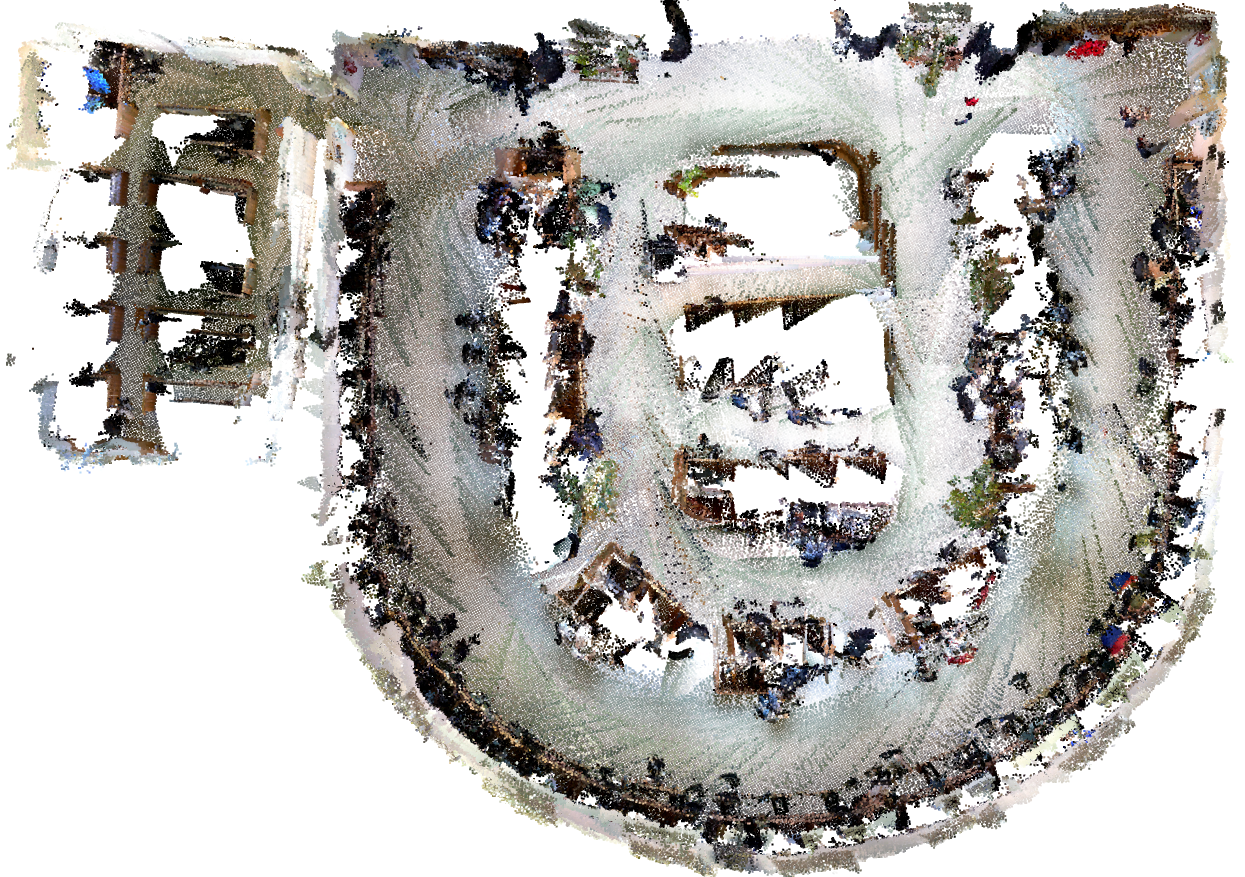
\includegraphics[width=\linewidth]{../img/mff_rotunda_2.png}
    \end{tikzfigure}
\end{minipage}
\hfill
\begin{minipage}[t]{0.33\linewidth}
    \begin{tikzfigure}
        \centering
        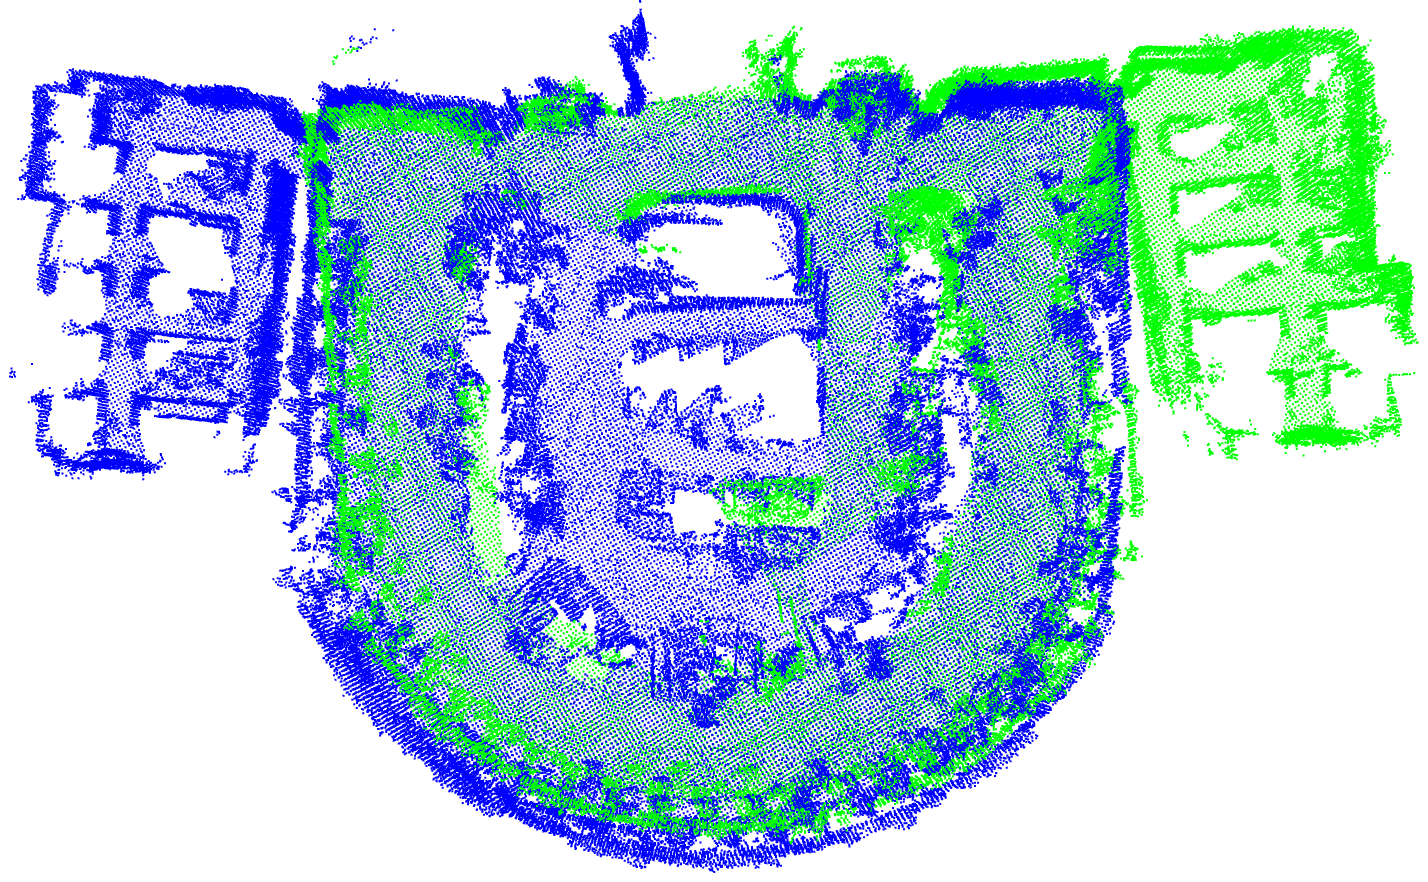
\includegraphics[width=\linewidth]{rotunda_merged.png}
\end{tikzfigure}
\end{minipage}
\hfill
\begin{minipage}[t]{0.27\linewidth}
    \begin{tikzfigure}
        \centering
        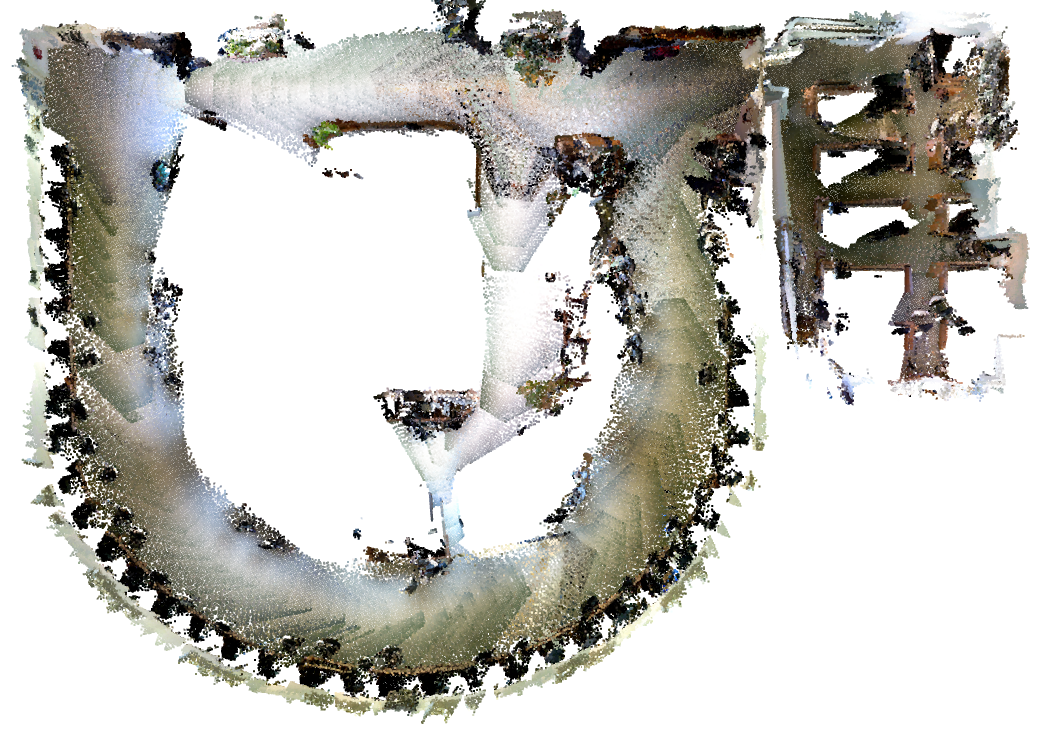
\includegraphics[width=\linewidth]{../img/mff_rotunda_1.png}
\end{tikzfigure}
\end{minipage}
} % end block
% \end{blockemph}

\block{Contribution}{
% \vspace{0.5em}
% \begin{minipage}[t]{0.74\linewidth}
\begin{itemize}[leftmargin=*,labelindent=0.5em,labelsep=1em,itemsep=0em,parsep=0em]
    \item The presented approach is the first implemented map-merging algorithm working directly on \textbf{point clouds without any auxiliary information}.
    \item The presented implementation is the \textbf{first implementation} of a \gls{3D} map-merging algorithm for multi-robot systems within the \gls{ROS} ecosystem.
    \item A \textbf{new reciprocal descriptor matching algorithm} was introduced for estimating the initial transformation using feature-matching.
\end{itemize}
% \vspace{0.5em}
} % end block

\block{ROS package}{
\vspace{0.5em}
\begin{minipage}[t]{0.50\linewidth}
The implementation presented in this work leverages modularity of the widely-used \gls{ROS} framework and respects community established standards. This allows easy integration with existing planning, mapping and communication algorithms enabling quick development of multi-robot systems suited for the particular task.

\vspace{1em}

This work has been accepted to the official \gls{ROS} distribution. It is available from \gls{ROS} Melodic.

\vspace {1em}

\begin{tabular}{ l l }
Source: &\url{https://github.com/hrnr/map-merge} \\
Wiki: &\url{http://wiki.ros.org/map_merge_3d}
\end{tabular}

\end{minipage}
\hfill
\begin{minipage}[t]{0.47\linewidth}

\begin{tikzfigure}
  \centering
  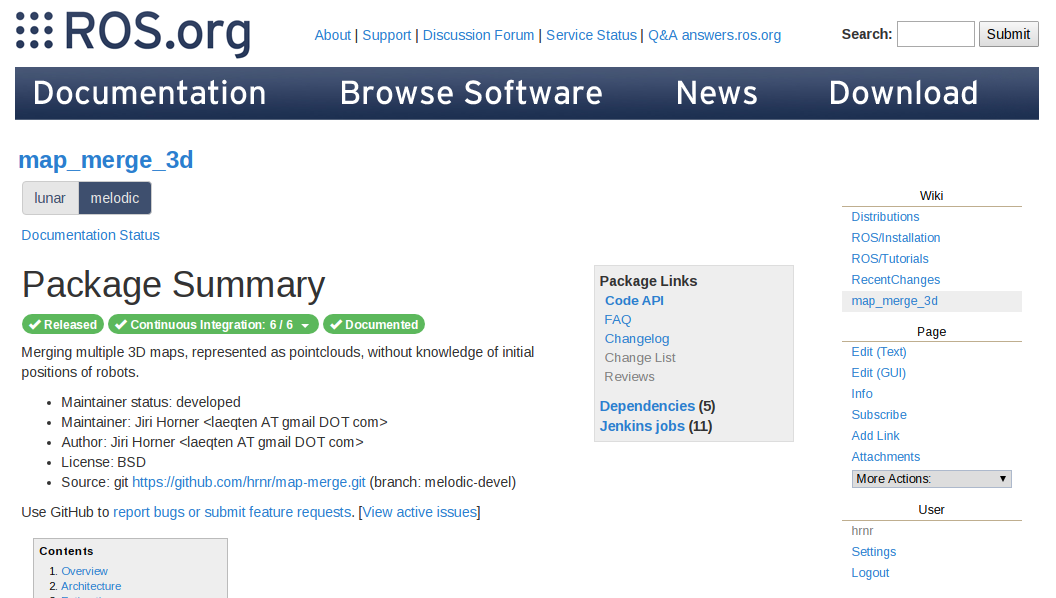
\includegraphics[width=\linewidth]{ros_wiki.png}
\end{tikzfigure}
\end{minipage}

% \vspace{0.5em}
} % end block

\column{0.5}

\block{Experiments and Results}{
\vspace{0.5em}

The map-merging algorithm has been evaluated on real-world datasets captured by both aerial and ground-based robots with a~variety of stereo rig cameras and active \gls{RGB-D} cameras. It has been evaluated in both indoor and outdoor environments ranging from forest to a single furnished room. The datasets used for evaluation include both well-established benchmark robotics datasets and my own experiments.

\begin{minipage}[t]{0.24\linewidth}
\begin{tikzfigure}
  \centering
  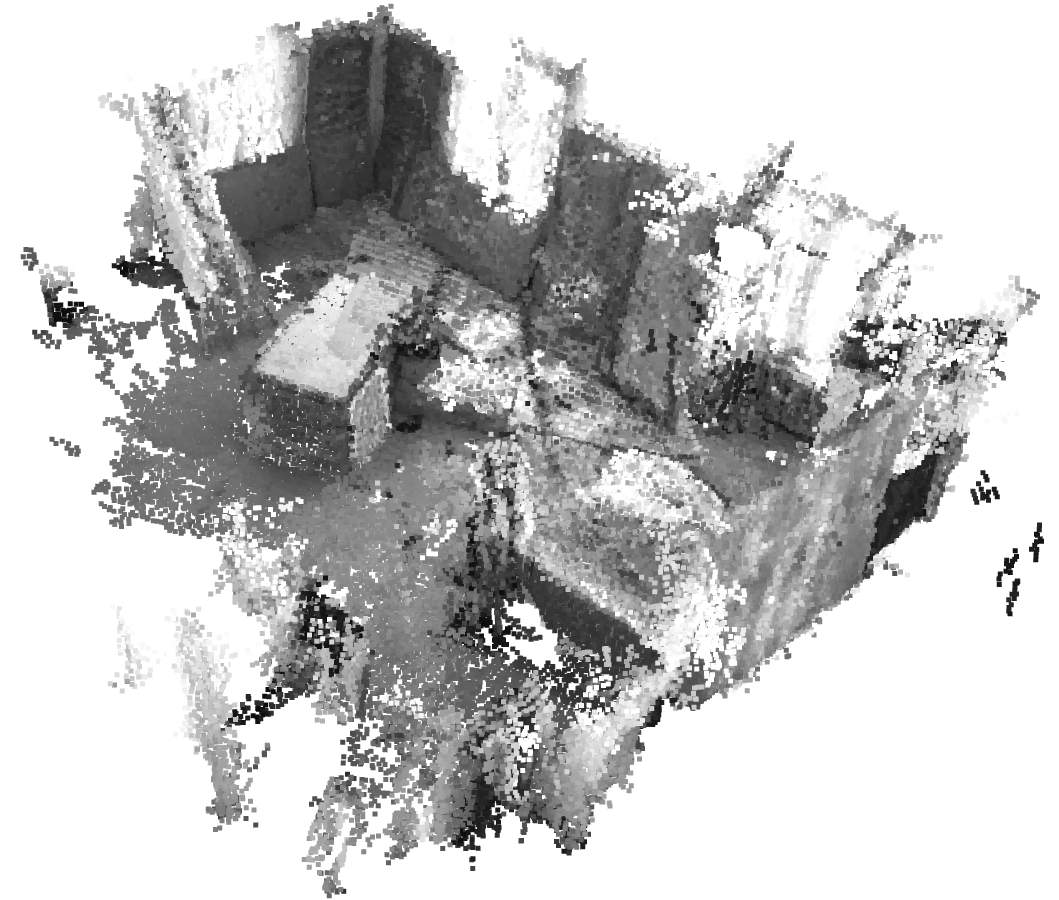
\includegraphics[width=\linewidth]{../img/v1-greyscale.png}
\end{tikzfigure}
\end{minipage}
\hfill
\begin{minipage}[t]{0.24\linewidth}
\begin{tikzfigure}
  \centering
  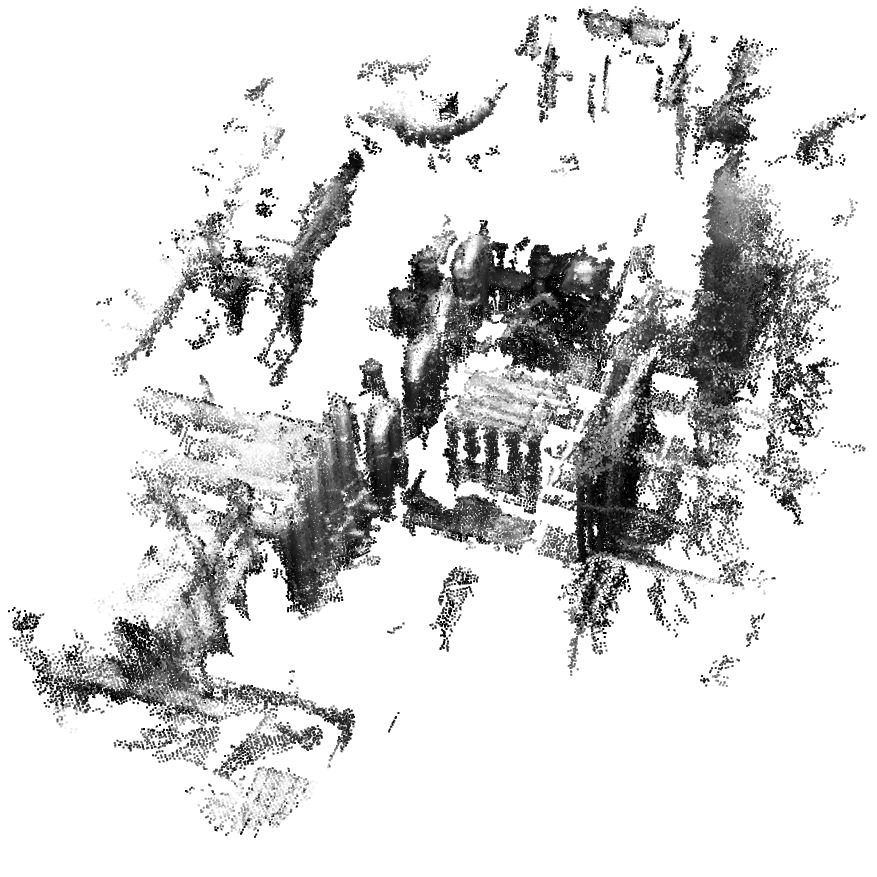
\includegraphics[width=\linewidth]{../img/euroc_mh_02.png}
\end{tikzfigure}
\end{minipage}
\hfill
\begin{minipage}[t]{0.24\linewidth}
\begin{tikzfigure}
  \centering
  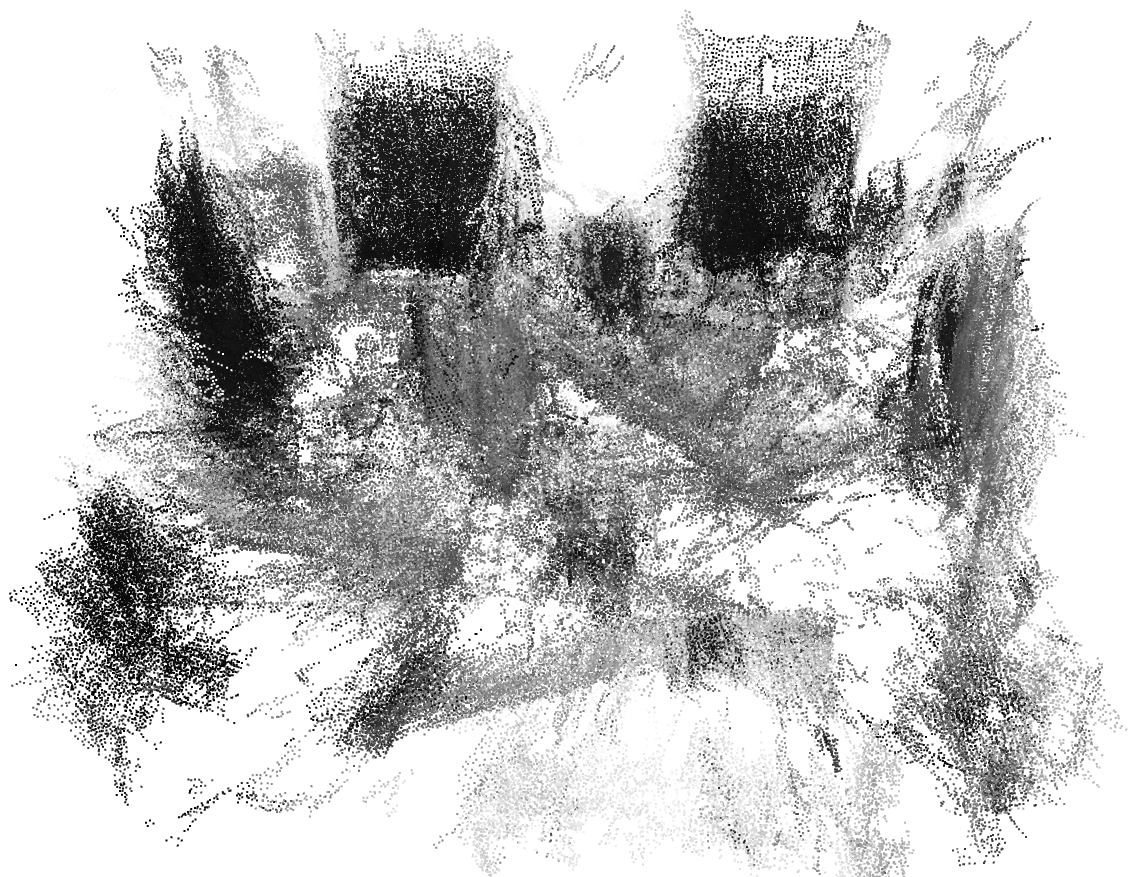
\includegraphics[width=\linewidth]{../img/euroc_v2_02.png}
\end{tikzfigure}
\end{minipage}
\hfill
\begin{minipage}[t]{0.24\linewidth}
\begin{tikzfigure}
  \centering
  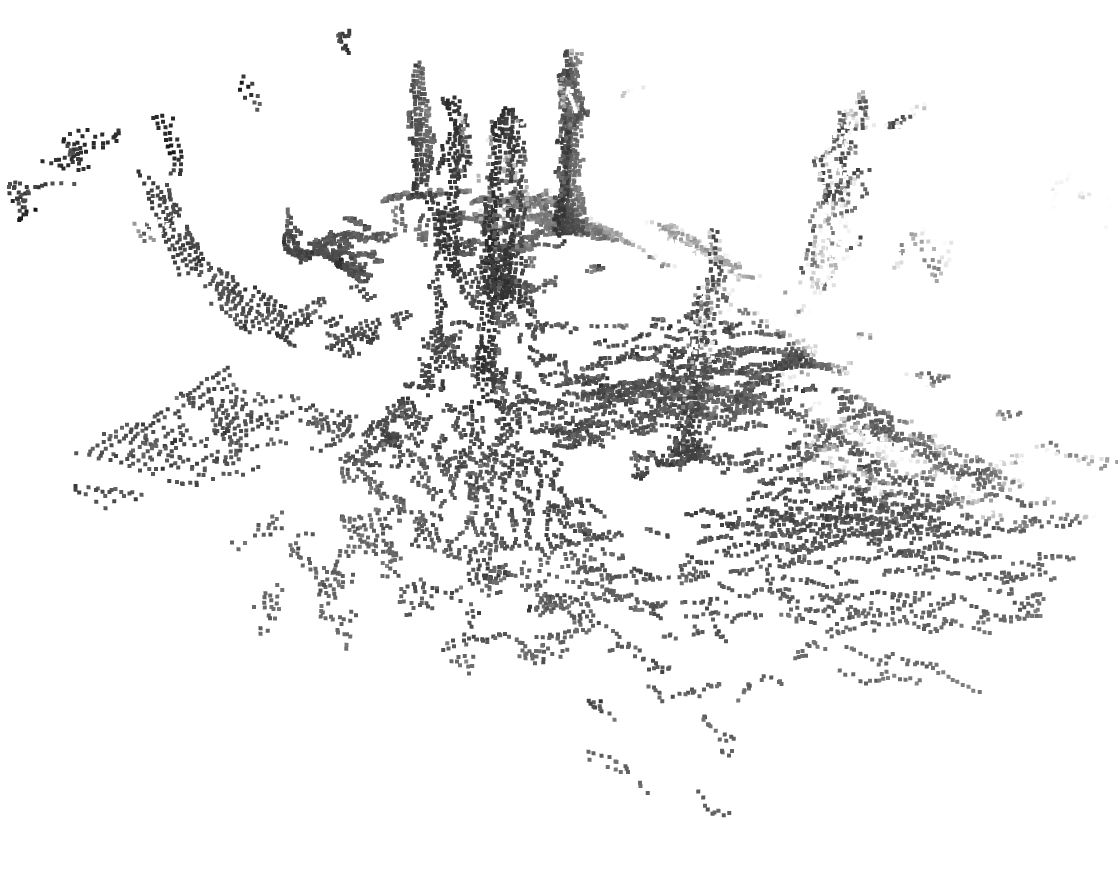
\includegraphics[width=\linewidth]{../img/aau_fc_dnav5_top.png}
\end{tikzfigure}
\end{minipage}

\begin{minipage}[t]{0.70\linewidth}
\begin{tikzfigure}
  \centering
  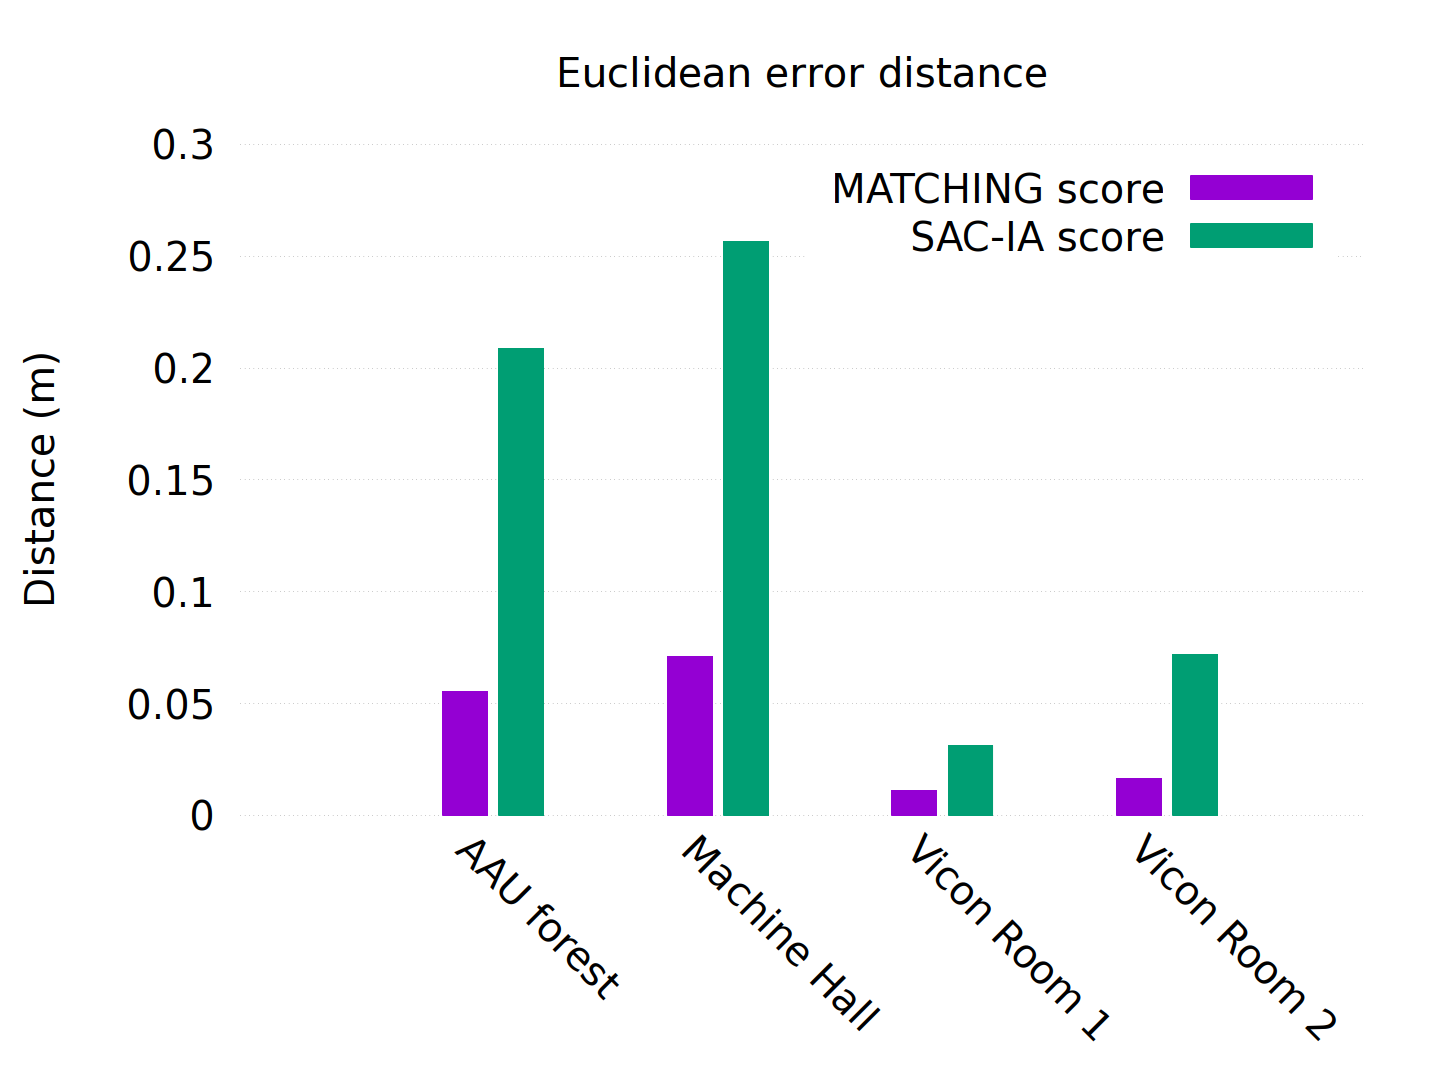
\includegraphics[width=\linewidth]{euc_dist_2.png}
\end{tikzfigure}
\end{minipage}
\begin{minipage}[t]{0.24\linewidth}
\begin{tikzfigure}
  \centering
  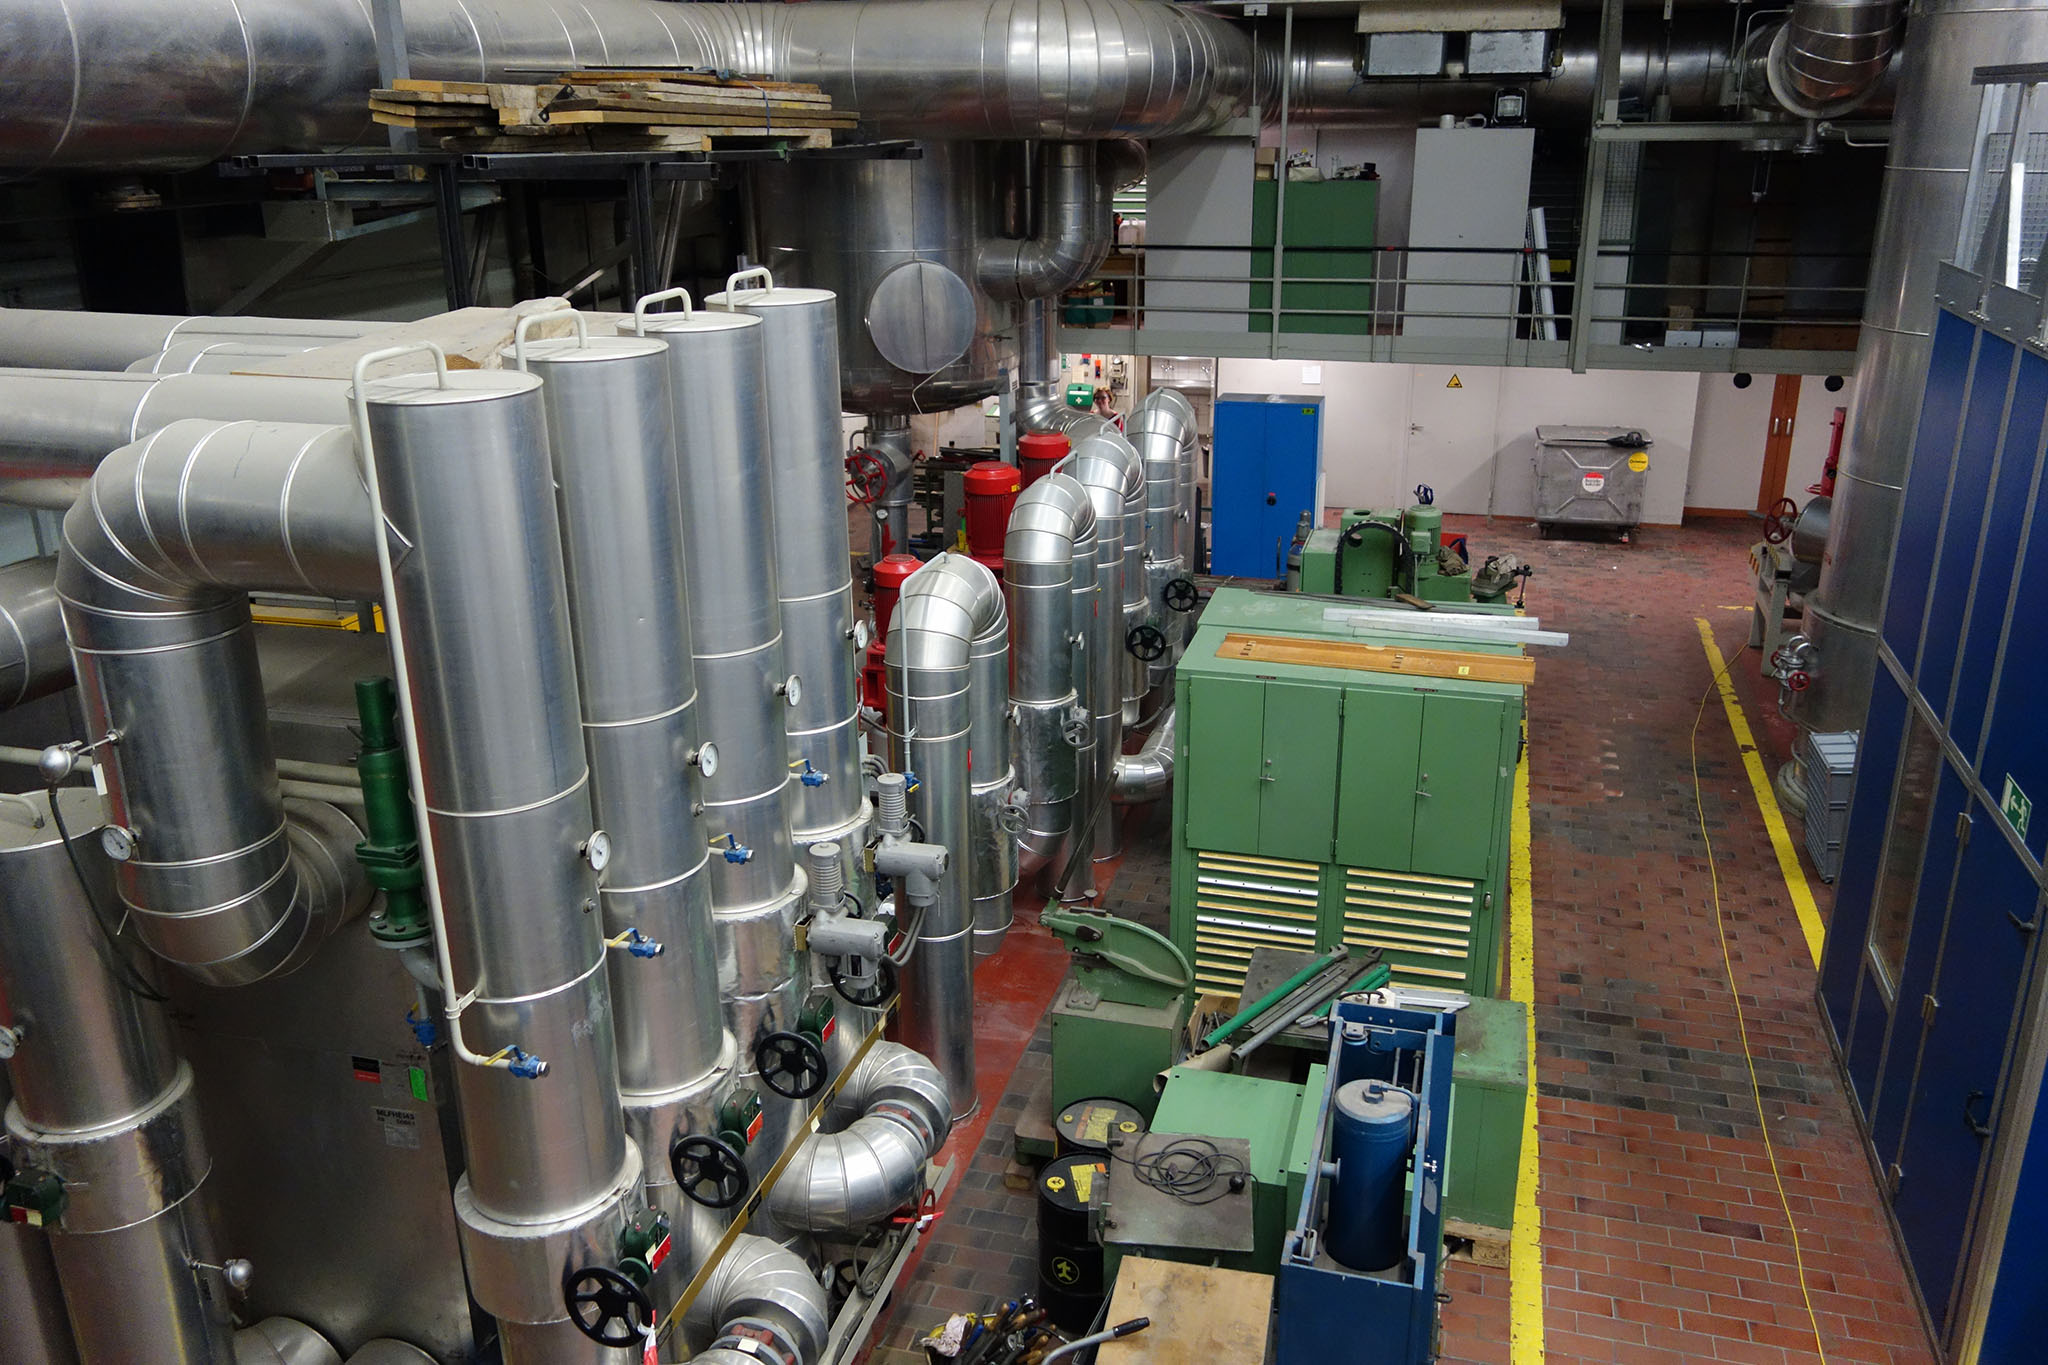
\includegraphics[width=\linewidth]{../img/eth_machine_room.jpg}
\end{tikzfigure}
\begin{tikzfigure}
  \centering
  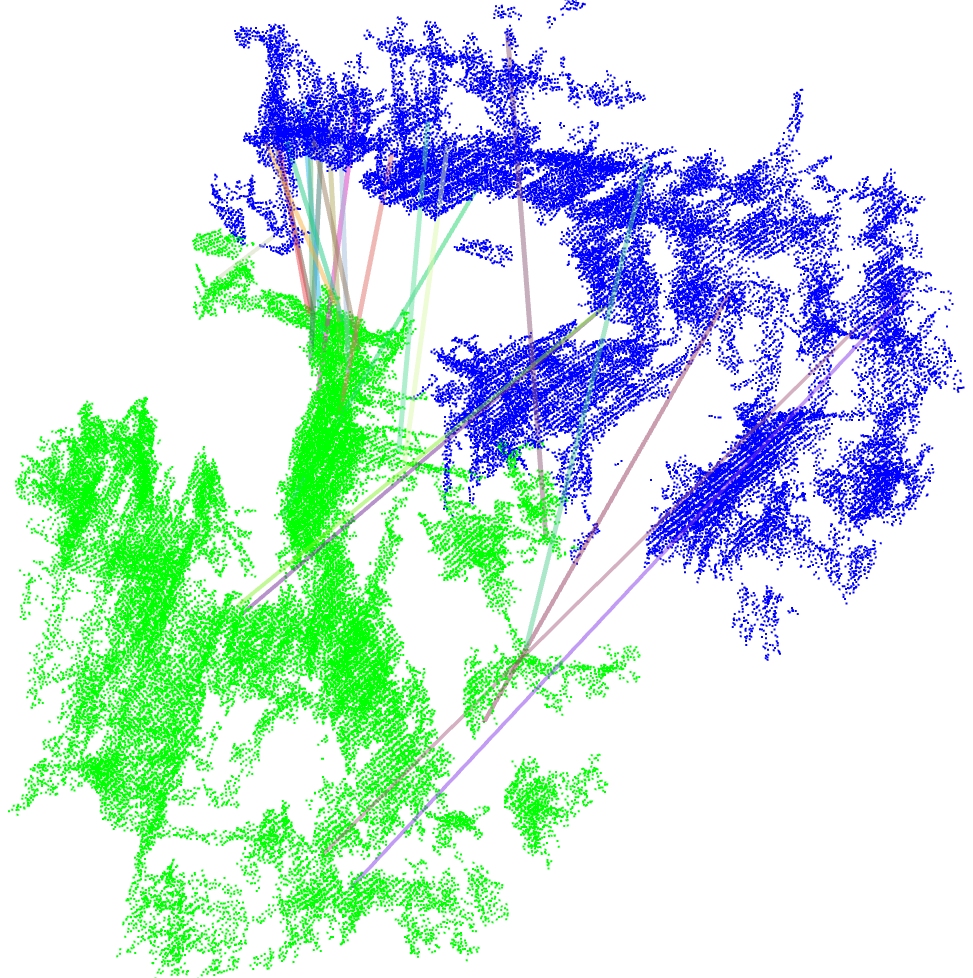
\includegraphics[width=\linewidth]{matches.png}
\end{tikzfigure}
\end{minipage}

In the most configurations, my new reciprocal matching scheme introduced in this work outperforms \gls{SAC-IA} algorithm for initial alignment available in the \gls{PCL}.

\vspace{1em}

The work showed the feasibility of the feature-matching approach for registration of low-density point cloud maps produced by~\gls{SLAM} algorithms while using \gls{3D} point cloud features typically employed with high-density sensor data. The presented algorithm is applicable in heterogeneous multi-robot systems and the algorithm can work with different \gls{SLAM} approaches and sensor types.

\vspace{0.3em}
} % end block

\end{columns}

\end{document}